\chapter{Конструкторская часть}
В данном разделе представлены последовательная и параллель­ная схемы алгоритма, 
описанного в аналитической части.


\section{Схемы алгоритмов}

На рисунке \ref{scheme:serial} представлена схема последовательного алгоритма
поворота точек в пространстве.
\begin{figure}[!htb]
	\centering
	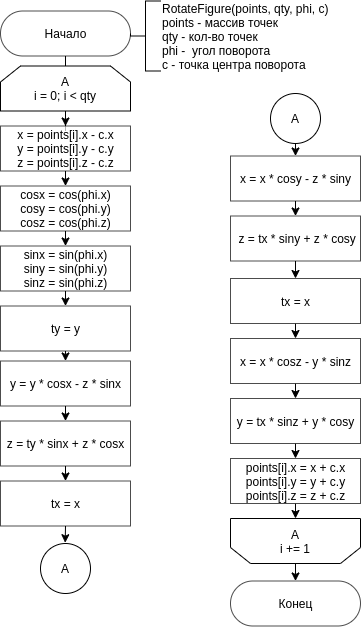
\includegraphics[scale=0.7]{schemes/serial}
	\caption{Схема последовательного алгоритма поворота точек}
	\label{scheme:serial}
\end{figure}

\newpage

На рисунке \ref{scheme:concur_abstr} представлена схема распараллеливания алгоритма
поворота точек двумерного растра.
\begin{figure}[!htb]
	\centering
	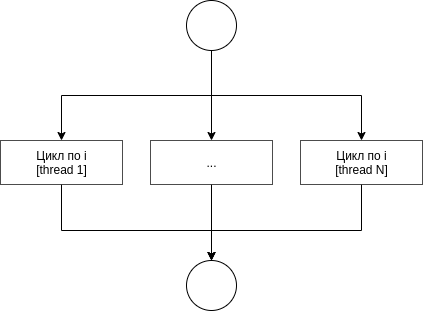
\includegraphics[scale=0.55]{schemes/concur_abstr}
	\caption{Схема распараллеливания алгоритма поворота точек}
	\label{scheme:concur_abstr}
\end{figure}


На рисунке \ref{scheme:concur} представлена схема паралелльного алгоритма
поворота точек в пространстве.
\begin{figure}[!htb]
	\centering
	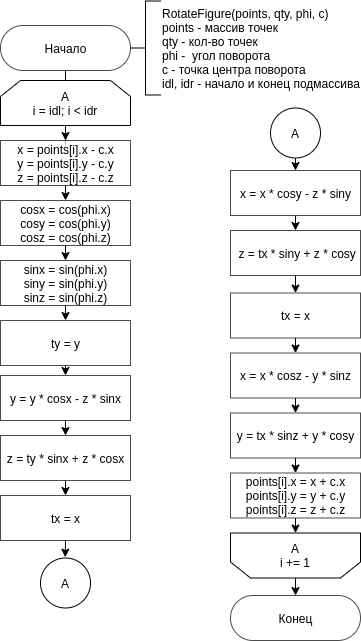
\includegraphics[scale=0.58]{schemes/concur}
	\caption{Схема параллельного алгоритма поворота точек}
	\label{scheme:concur}
\end{figure}


На рисунке \ref{scheme:threaddistr} представлена схема функции создания потоков и
запуска параллельных реализаций вычислений
\begin{figure}[!htb]
	\centering
	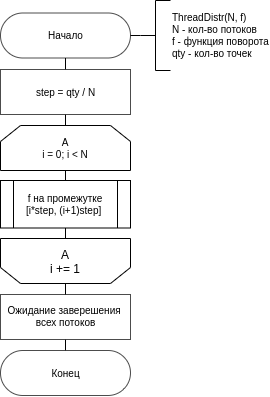
\includegraphics[scale=0.58]{schemes/threaddistr}
	\caption{Схема параллельного алгоритма поворота точек}
	\label{scheme:threaddistr}
\end{figure}


\section{Выделение классов эквивалентности}

Для тестирования программы были выделены следующие классы эквивалентности:
\begin{itemize}
    \item поворот на нулевой угол;
    \item поворот на положительный угол;
    \item поворот на отрицательный угол;
    \item ни одной точки на вход;
    \item одна точка на вход;
    \item несколько точек на вход;
    \item выбран 1 поток исполнения;
    \item выбрано несколько потоков исполнения;
    \item выбрано 0 потоков исполнения;
    \item некорректные координаты точки;
    \item некорректный угол поворота.
\end{itemize}

\section{Вывод}
На основе теоретических данных, полученных из аналитического
раздела, были разработаны схемы требуемых алгоритмов, а также выделены классы
эквивалентности для последующего функционального тестирования.
